% !TEX TS-program = pdflatex
% !TEX encoding = UTF-8 Unicode

% This is a simple template for a LaTeX document using the "article" class.
% See "book", "report", "letter" for other types of document.

% \documentclass[11pt]{article} % use larger type; default would be 10pt
\documentclass[
    10pt, % Schriftgröße
    DIV12,
    english, % für Umlaute, Silbentrennung etc.
    a5paper, % Papierformat
    twoside, % zweiseitiges Dokument
    titlepage, % es wird eine Titelseite verwendet
    parskip=half, % Abstand zwischen Absätzen (halbe Zeile)
    headings=small, % Größe der Überschriften verkleinern
    listof=totoc, % Verzeichnisse im Inhaltsverzeichnis aufführen
    bibliography=totoc, % Literaturverzeichnis im Inhaltsverzeichnis aufführen
    index=totoc, % Index im Inhaltsverzeichnis aufführen
    captions=tableheading, % Beschriftung von Tabellen unterhalb ausgeben
    final % Status des Dokuments (final/draft)
]{scrbook}

\usepackage[utf8]{inputenc} % set input encoding (not needed with XeLaTeX)
\usepackage[T1]{fontenc}
\usepackage{textcomp} % Euro-Zeichen etc.

\usepackage[
	automark, % Kapitelangaben in Kopfzeile automatisch erstellen
	headsepline, % Trennlinie unter Kopfzeile
	ilines % Trennlinie linksbündig ausrichten
]{scrlayer-scrpage}

% Anpassung an Landessprache ---------------------------------------------------
\usepackage[english]{babel}

%%% Examples of Article customizations
% These packages are optional, depending whether you want the features they provide.
% See the LaTeX Companion or other references for full information.

\usepackage{lmodern} % bessere Fonts
\usepackage{relsize} % Schriftgröße relativ festlegen

%%% PAGE DIMENSIONS
% \usepackage{geometry} % to change the page dimensions
\usepackage{setspace}
\usepackage[paperwidth=17cm,paperheight=24cm]{geometry}
% \geometry{a4paper} % or letterpaper (US) or a5paper or....
% \geometry{margin=2in} % for example, change the margins to 2 inches all round
% \geometry{landscape} % set up the page for landscape
%   read geometry.pdf for detailed page layout information
\geometry{left=20mm,right=20mm,top=15mm,bottom=20mm}

\usepackage{graphicx} % support the \includegraphics command and options

% \usepackage[parfill]{parskip} % Activate to begin paragraphs with an empty line rather than an indent

%%% PACKAGES
\usepackage{trfsigns}
\usepackage{booktabs} % for much better looking tables
\usepackage{array} % for better arrays (eg matrices) in maths
\usepackage{paralist} % very flexible & customisable lists (eg. enumerate/itemize, etc.)
\usepackage{verbatim} % adds environment for commenting out blocks of text & for better verbatim
\usepackage{subfig} % make it possible to include more than one captioned figure/table in a single float
\usepackage{float}
\usepackage{amsmath} %
\usepackage{amssymb}
\usepackage{tikz} % Draw sig­nal flow graphs
\usetikzlibrary{dsp,chains}
% These packages are all incorporated in the memoir class to one degree or another...

%%% HEADERS & FOOTERS
% \usepackage{fancyhdr} % This should be set AFTER setting up the page geometry
% \pagestyle{fancy} % options: empty , plain , fancy
% \renewcommand{\headrulewidth}{0pt} % customise the layout...
% \lhead{}\chead{}\rhead{}
% \lfoot{}\cfoot{\thepage}\rfoot{}

% Kopf- und Fußzeilen ----------------------------------------------------------
\pagestyle{scrheadings}
% Kopf- und Fußzeile auch auf Kapitelanfangsseiten
\renewcommand*{\chapterpagestyle}{scrheadings} 
% Schriftform der Kopfzeile
\renewcommand{\headfont}{\normalfont}

% Kopfzeile
\ihead{\textit{\headmark}}
\chead{}
\ohead{\pagemark}
\setlength{\headheight}{10mm} % Höhe der Kopfzeile
\setheadsepline[text]{0.4pt} % Trennlinie unter Kopfzeile

% Fußzeile
\ifoot{}
\cfoot{}
\ofoot{}

\setlength{\footskip}{20pt}

%%% SECTION TITLE APPEARANCE
%\usepackage{sectsty}
%\allsectionsfont{\sffamily\mdseries\upshape} % (See the fntguide.pdf for font help)
% (This matches ConTeXt defaults)

\RedeclareSectionCommand[
  beforeskip=-1sp,
  afterskip=2\baselineskip]{chapter}
\RedeclareSectionCommand[
  beforeskip=-\baselineskip,
  afterskip=.5\baselineskip]{section}
\RedeclareSectionCommand[
  beforeskip=-.75\baselineskip,
  afterskip=.5\baselineskip]{subsection}
\RedeclareSectionCommand[
  beforeskip=-.5\baselineskip,
  afterskip=.25\baselineskip]{subsubsection}
\RedeclareSectionCommand[
  beforeskip=.5\baselineskip,
  afterskip=-1em]{paragraph}
\RedeclareSectionCommand[
  beforeskip=-.5\baselineskip,
  afterskip=-1em]{subparagraph}

%%% ToC (table of contents) APPEARANCE
\usepackage[nottoc,notlof,notlot]{tocbibind} % Put the bibliography in the ToC
\usepackage[titles,subfigure]{tocloft} % Alter the style of the Table of Contents
\renewcommand{\cftsecfont}{\rmfamily\mdseries\upshape}
\renewcommand{\cftsecpagefont}{\rmfamily\mdseries\upshape} % No bold!

\DeclareMathAlphabet{\mathpzc}{OT1}{pzc}{m}{it}
\newcommand{\z}{\mathpzc{z}}

\usepackage{xcolor}
\definecolor{instruction}{gray}{0.80}

\newtheorem{beispiel}{Beispiel}[chapter]

% zum Einbinden von Programmcode -----------------------------------------------
\usepackage{listings}
\usepackage{xcolor} 
\definecolor{hellgelb}{rgb}{1,1,0.9}
\definecolor{colKeys}{rgb}{0,0,1}
\definecolor{colIdentifier}{rgb}{0,0,0}
\definecolor{colComments}{rgb}{1,0,0}
\definecolor{colString}{rgb}{0,0.5,0}
\definecolor{hellgrau}{rgb}{0.96,0.96,0.96}
\lstset{
    float=hbp,
    basicstyle=\ttfamily\color{black}\small\smaller,
    identifierstyle=\color{black},
    keywordstyle=\color{black},
    stringstyle=\color{black},
    commentstyle=\color{gray},
    columns=flexible,
    tabsize=2,
    frame=single,
    extendedchars=true,
    showspaces=false,
    showstringspaces=false,
    numbers=left,
    numberstyle=\tiny,
    breaklines=true,
    backgroundcolor=\color{hellgrau},
    breakautoindent=true
}

%%% END Article customizations


%%% The "real" document content comes below...

%\title{Ausgewählte Themen der Informatik in Theorie und Praxis}
%\author{Jens Thielemann}
%\date{} % Activate to display a given date or no date (if empty),
         % otherwise the current date is printed 

\newcommand{\microphone}{%
    \tikz{
        \begin{scope}
            \clip (-.3em,-.4ex) rectangle (1.3em,1.5ex);
            \fill[black, rounded corners=1.5ex] (-.3em,-.4ex) rectangle (1.3em,5.5ex);
        \end{scope}
        \fill[white, rounded corners=1.3ex] (-.1em,0) rectangle (1.1em,5.1ex);
        \fill[black, rounded corners=1.1ex] (0,.2ex) rectangle (1em,5ex);
        \foreach \pos in {2.5ex, 2.9ex, 3.3ex, 3.7ex}
            \fill[white, rounded corners=.1ex] (.35em,\pos) rectangle +(.8em,.25ex);
        \fill[black] (.4em,-.4ex) rectangle (.6em,-1.5ex);
        \fill[black] (0,-1.5ex) rectangle (1em,-2ex);
    }%
}

\begin{document}
%\maketitle
\tableofcontents 

\newpage

\chapter{Apative Filter}

\section{Filter structure}
\begin{figure}[htbp]
\begin{tikzpicture}
	% Place nodes using a matrix
	\matrix (m1) [row sep=2.5mm, column sep=5mm]
	{
		%--------------------------------------------------------------------
		\node[coordinate]                  (m00) {};          &
		\node[coordinate]                  (m01) {};          &
		\node[coordinate]                  (m02) {};          &
		\node[coordinate]                  (m03) {};          &
		\node[coordinate]                  (m04) {};          &
		\node[coordinate]                  (m05) {};          &
		\node[dspnodeopen,dsp/label=above] (m06) {$d_k$};    &
		\node[coordinate]                  (m07) {};          &
		\node[coordinate]                   (m08) {}; &
		\node[coordinate]                   (m09) {};          \\
		%--------------------------------------------------------------------
		\\
		\\
		%--------------------------------------------------------------------
		\node[dspnodeopen,dsp/label=above] (m20) {$x_k$};    &
		\node[coordinate]                  (m21) {};          &
		\node[dspnodefull]                  (m22) {};          &
		\node[coordinate]                  (m23) {};          &
		\node[dspsquare, minimum size=1cm, , inner xsep=10pt]                  (m24) {Predictor};          &
		\node[coordinate]                 (m25) {};          &
		\node[dspadder]                    (m26) {};          &
		\node[dspnodefull]                 (m27) {};          &
		\node[coordinate]                   (m28) {}; &
		\node[dspnodeopen,dsp/label=above]  (m29) {$e_k$};          \\
		%--------------------------------------------------------------------
		\\
		\\
		%--------------------------------------------------------------------
		\node[coordinate]                  (m40) {};          &
		\node[coordinate]                  (m41) {};          &
		\node[coordinate]                  (m42) {};          &
		\node[coordinate]                  (m43) {};          &
		\node[dspfilter, minimum size=1.2cm, text height=2em, inner xsep=10pt]                  (m44) {Update\\ algorithm};          &
		\node[coordinate]                    (m45) {};          &
		\node[coordinate]                    (m46) {};          &
		\node[coordinate]                    (m47) {};          &
		\node[coordinate]                    (m48) {};          &
		\node[coordinate]                    (m49) {};          \\
		%--------------------------------------------------------------------
	};
	\draw[dspflow] (m20) -- (m22);
	\draw[dspconn] (m22) -- (m24);
	\draw[dspflow] (m27) -- (m29);
          \draw[dspline] (m22) -- (m42);
	\draw[dspconn] (m42) -- (m44);
           \draw[dspflow] (m24) -- node[midway,above] {$-\hat{x}_k$} (m26);
	\draw[dspline] (m27) -- (m47);
	\draw[dspline] (m26) -- (m27);
	\draw[dspconn] (m47) -- (m44);
	\draw[dspflow] (m06) -- (m26);
           \draw[dspconn] (m44) -- node[midway,right] {$\textit{\textbf{b}}_{k+1}$} (m24);
\end{tikzpicture}
\end{figure}

\section{Predictor}

\begin{equation}
\hat{x}_k=\sum_{i=0}^{N} b_i\:x_{k-i}\nonumber
\end{equation}

\begin{equation}
H(z)=\frac{\hat{X}(z)}{X(z)}=\sum_{i=0}^{N} b_i\:z^{-i}=b_0+b_1z^{-1}+\dots+b_N+z^{-N}\nonumber
\end{equation}

\begin{figure}[htbp]
\begin{tikzpicture}
	% Place nodes using a matrix
	\matrix (m1) [row sep=2.5mm, column sep=5mm]
	{
		%--------------------------------------------------------------------
		\node[dspnodeopen,dsp/label=above] (m00) {$x_k$};    &
		\node[coordinate]                  (m01) {};          &
		\node[dspnodefull]                 (m02) {};          &
		\node[dspsquare]                   (m03) {$\z^{-1}$}; &
		\node[dspnodefull]                 (m04) {};          &
		\node[dspsquare]                   (m05) {$\z^{-1}$}; &
		\node[dspnodefull]                 (m06) {};          &
		\node[dspsquare]                   (m07) {$\z^{-1}$}; &
		\node[coordinate]                  (m08) {};          &
		\node[coordinate]                  (m09) {};          &
		\node[coordinate]                  (m0X) {};          \\
		%--------------------------------------------------------------------
		\\
		\\
		%--------------------------------------------------------------------
		\node[coordinate]                  (m20) {};          &
		\node[coordinate]                  (m21) {};          &
		\node[coordinate]                  (m22) {};          &
		\node[coordinate]                  (m23) {};          &
		\node[dspadder]                    (m24) {};          &
		\node[coordinate]                  (m25) {};          &
		\node[dspadder]                    (m26) {};          &
		\node[coordinate]                  (m27) {};          &
		\node[dspadder]                    (m28) {};          &
		\node[coordinate]                  (m29) {};          &
		\node[dspnodeopen,dsp/label=above] (m2X) {$\hat{x}_k$};    \\
		%--------------------------------------------------------------------
	};
	\draw[dspflow] (m00) -- (m02);
	\draw[dspconn] (m02) -- (m03);
	\draw[dspflow] (m02) -- node[midway,right] {$b_0$} (m22);
          \draw[dspconn] (m22) -- (m24);
          \draw[dspconn] (m03) -- (m05);
          	\draw[dspflow] (m04) -- node[midway,right] {$b_1$} (m24);
          \draw[dspconn] (m05) -- (m07);
          	\draw[dspflow] (m06) -- node[midway,right] {$b_2$} (m26);
          \draw[dspconn] (m24) -- (m26);
          \draw[dspconn] (m26) --  (m28);
          	\draw[dspflow] (m08) -- node[midway,right] {$b_3$} (m28);
          	\draw[dspflow] (m28) -- (m2X);
          \draw[dspline] (m07) -- (m08);
\end{tikzpicture}
\end{figure}

\begin{equation}\label{error}
e_k=d_k-\hat{x}_k
\end{equation}

\section{Update Algorithm}

Least Mean Square algorithm

\begin{figure}[H]
\centering
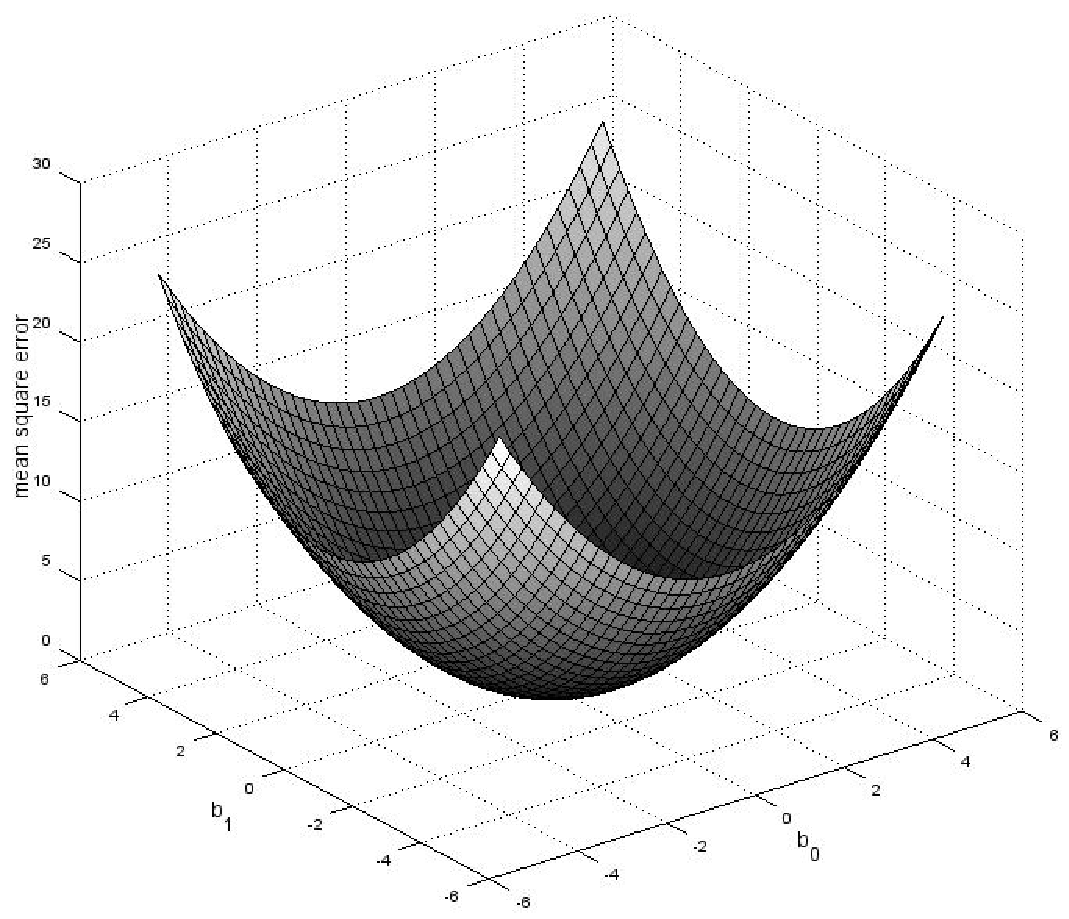
\includegraphics[width=10cm]{../Images/mse.pdf}
\end{figure}

\begin{equation}
\textit{\textbf{b}}_{k+1}=\textit{\textbf{b}}_k-\beta \frac{\partial E(e_k^2)}{\partial \textit{\textbf{b}}_k}\nonumber
\end{equation}

\begin{equation}
E(e_k^2) = \frac{1}{N}\sum_{k=0}^{N-1}\left(x_k-\textit{\textbf{b}}_k\textit{\textbf{X}}_k\right)^2=E\left(\left(x_k-\textit{\textbf{b}}_k\textit{\textbf{X}}_k\right)^2\right) \nonumber
\end{equation}

\begin{equation}
E(e_k^2) = E(x_k^2)-2\textit{\textbf{b}}_k E(\textit{\textbf{X}}_k)+\textit{\textbf{b}}_k^T E(\textit{\textbf{X}}_k^2)\textit{\textbf{b}}_k\nonumber
\end{equation}

\begin{equation}
\frac{\partial E(e_k^2) }{\partial \textit{\textbf{b}}_k}= -2 E(\textit{\textbf{X}}_k)+2 \textit{\textbf{b}}_k E(\textit{\textbf{X}}_k^2)\nonumber
\end{equation}

\begin{equation}
\frac{\partial E(e_k^2) }{\partial \textit{\textbf{b}}_k}= -2 \underbrace{E(\textit{\textbf{X}}_k)}_\text{\clap{mean value free}}+2 \textit{\textbf{b}}_k \underbrace{E(\textit{\textbf{X}}_k^2)}_\text{\clap{$R_{xx,k}$}}\nonumber
\end{equation}

\begin{equation}
\frac{\partial E(e_k^2)}{\partial \textit{\textbf{b}}_k}=2\textit{\textbf{R}}_{xx,k}\textit{\textbf{b}}_k\nonumber
\end{equation}

\begin{equation}
\frac{\partial E(e_k^2)}{\partial \textit{\textbf{b}}_k} \approx \frac{\Delta E(e_k^2)}{\Delta \textit{\textbf{b}}_k}=2\textit{\textbf{R}}_{xx,k}\left(\textit{\textbf{b}}_k-\textit{\textbf{b}}_{k-1}\right)\nonumber
\end{equation}

\begin{equation}
\textit{\textbf{b}}_{k+1}=\textit{\textbf{b}}_k-2\beta \textit{\textbf{R}}_{xx,k}\left(\textit{\textbf{b}}_k-\textit{\textbf{b}}_{k-1}\right)\nonumber
\end{equation}

Optimum reached/exceeded by
\begin{equation}
\frac{\textit{\textbf{b}}_{k+1}-\textit{\textbf{b}}_{k}}{\textit{\textbf{b}}_{k}-\textit{\textbf{b}}_{k-1}}\leq 0 \rightarrow -1\nonumber
\end{equation}


\begin{equation}
\beta=\frac{1}{2}\:I\:\textit{\textbf{R}}_{xx,k}^{-1} \xrightarrow{n\:x\:n} \beta=\frac{1}{2}\:\textit{\textbf{R}}_{xx,k}^{-1}\nonumber
\end{equation}

\begin{equation}
0 < \beta < \textit{\textbf{R}}_{xx,k}^{-1} \nonumber
\end{equation}
Convergence at sum of $\textit{\textbf{R}}_{xx,k}$  intrinsic values 
\begin{equation}
(N+1)\:R_{xx}(0)=(N+1)\:\sigma_{xx}^2\nonumber
\end{equation}

\begin{equation}
0 < \beta < \frac{1}{(N+1)\:\sigma_{xx}^2} \nonumber
\end{equation}

\section{Noise and Echo cancellation}



\chapter{Prädiktion}
Viele Aufgaben in der digitalen Signalverarbeitung werden mit der Prädiktion realisiert. Dazu zählen Anwendungen in der Audio- und Videocodierung, Vorhersagen von Aktienkursen, 
Störunterdrückung und überall dort wo Schätzungen von Signalwerten durchgeführt werden müssen.

\section{Linearer Prädiktor}
Die Prädiktion schätzt mittels Linearkombination aus einem vorangegangenen Signal neue Werte. Die Linearkombination kann 
durch folgende Differenzengleichung ausgedrückt werden:
\begin{equation}\label{linearcombination}
\hat{x}_k=\sum_{i=0}^{N} b_i\:x_{k-i}
\end{equation}
Die zugehörige zeitdiskrete Übertragungsfunktion lautet nach der z-Transformation:
\begin{equation}
H(z)=\frac{\hat{X}(z)}{X(z)}=\sum_{i=0}^{N} b_i\:z^{-i}=b_0+b_1z^{-1}+\dots+b_N+z^{-N}\nonumber
\end{equation}
Diese Übertragungsfunktion lässt sich auch als FIR-Filter mit der zugehörigen Struktur hier als Beispiel mit N=3 dargestellen:\\
\begin{figure}[htbp]
\centering
\begin{tikzpicture}
	% Place nodes using a matrix
	\matrix (m1) [row sep=2.5mm, column sep=5mm]
	{
		%--------------------------------------------------------------------
		\node[dspnodeopen,dsp/label=above] (m00) {$x_k$};    &
		\node[coordinate]                  (m01) {};          &
		\node[dspnodefull]                 (m02) {};          &
		\node[dspsquare]                   (m03) {$\z^{-1}$}; &
		\node[dspnodefull]                 (m04) {};          &
		\node[dspsquare]                   (m05) {$\z^{-1}$}; &
		\node[dspnodefull]                 (m06) {};          &
		\node[dspsquare]                   (m07) {$\z^{-1}$}; &
		\node[coordinate]                  (m08) {};          &
		\node[coordinate]                  (m09) {};          &
		\node[coordinate]                  (m0X) {};          \\
		%--------------------------------------------------------------------
		\\
		\\
		%--------------------------------------------------------------------
		\node[coordinate]                  (m20) {};          &
		\node[coordinate]                  (m21) {};          &
		\node[coordinate]                  (m22) {};          &
		\node[coordinate]                  (m23) {};          &
		\node[dspadder]                    (m24) {};          &
		\node[coordinate]                  (m25) {};          &
		\node[dspadder]                    (m26) {};          &
		\node[coordinate]                  (m27) {};          &
		\node[dspadder]                    (m28) {};          &
		\node[coordinate]                  (m29) {};          &
		\node[dspnodeopen,dsp/label=above] (m2X) {$\hat{x}_k$};    \\
		%--------------------------------------------------------------------
	};
	\draw[dspflow] (m00) -- (m02);
	\draw[dspconn] (m02) -- (m03);
	\draw[dspflow] (m02) -- node[midway,right] {$b_0$} (m22);
          \draw[dspconn] (m22) -- (m24);
          \draw[dspconn] (m03) -- (m05);
          	\draw[dspflow] (m04) -- node[midway,right] {$b_1$} (m24);
          \draw[dspconn] (m05) -- (m07);
          	\draw[dspflow] (m06) -- node[midway,right] {$b_2$} (m26);
          \draw[dspconn] (m24) -- (m26);
          \draw[dspconn] (m26) --  (m28);
          	\draw[dspflow] (m08) -- node[midway,right] {$b_3$} (m28);
          	\draw[dspflow] (m28) -- (m2X);
          \draw[dspline] (m07) -- (m08);
\end{tikzpicture}
\caption{FIR-Filterstruktur für N=3}
\end{figure}\\
Um das Prädiktionsfilter auf dessen Genauigkeit beurteilen zu können wird der Originalwert $x_k$ mit dem geschätzten Wert $\hat{x}_k$ verglichen. In Abbildung \ref{fig:linearpredictor} 
wird die FIR-Filterstruktur als Übertragungsfunktion $H(z)$ dargestellt.\\
\begin{figure}[htbp]
\centering
\begin{tikzpicture}
	% Place nodes using a matrix
	\matrix (m1) [row sep=2.5mm, column sep=5mm]
	{
		%--------------------------------------------------------------------
		\node[dspnodeopen,dsp/label=above] (m00) {$x_k$};    &
		\node[coordinate]                  (m01) {};          &
		\node[dspnodefull]                 (m02) {};          &
		\node[coordinate]                   (m03) {}; &
		\node[dspadder]                    (m04) {};          &
		\node[coordinate]                   (m05) {}; &
		\node[dspnodeopen,dsp/label=above]  (m06) {$e_k$};          \\
		%--------------------------------------------------------------------
		\\
		\\
		%--------------------------------------------------------------------
		\node[coordinate]                  (m20) {};          &
		\node[coordinate]                  (m21) {};          &
		\node[coordinate]                  (m22) {};          &
		\node[dspsquare]                  (m23) {$\:H(z)\:$};          &
		\node[coordinate]                    (m24) {};          &
		\node[coordinate]                    (m25) {};          &
		\node[coordinate]                    (m26) {};          \\
		%--------------------------------------------------------------------
	};
	\draw[dspflow] (m00) -- (m02);
	\draw[dspconn] (m02) -- (m04);
	\draw[dspflow] (m04) -- (m06);
          \draw[dspline] (m02) -- (m22);
	\draw[dspconn] (m22) -- (m23);
          \draw[dspline] (m23) -- (m24);
	\draw[dspconn] (m24) -- node[midway,right] {$-\hat{x}_k$} (m04);
\end{tikzpicture}
\caption{Struktur eines linearen Prädiktors}
\label{fig:linearpredictor}
\end{figure}\\
Im Idealfall ist die Differenz aus bekanntem Wert und dem geschätzten Wert gleich Null. 
In Realität jedoch erhält man einen Fehlerwert 
\begin{equation}\label{error}
e_k=x_k-\hat{x}_k
\end{equation}

\raggedbottom

\section{Bestimmung des Schätzfehlers}
An zentraler Stelle steht zur Bestimmung von Schätzwerten die Berechnung des Erwartungswertes. Der Erwartungswert bescheibt allgemein den Mittelwert einer Wertefolge 
$\textit{\textbf{X}}$:
\begin{equation}
E(\textit{\textbf{X}})=\sum_{i=0}^{N-1} p_i\:x_i\nonumber
\end{equation}
Wobei $p_i$ die Wahrscheinlichkeit eines Wertes der Wertefolge darstellt. Für Erwartungswerte eines Produktes aus 2 stochastik unabhängigen Wertefolgen 
$\textit{\textbf{X}}_i$ und $\textit{\textbf{X}}_j$ 
gilt der Zusammenhang:
\begin{equation}\label{twovariables}
E(\textit{\textbf{X}}_i\textit{\textbf{X}}_j)=\sum_{i=0}^{N-1}\sum_{j=0}^{N-1} p_i\:p_j\:x_i\:x_j
\end{equation}
Handelt es sich bei einer Wertefolge $\textit{\textbf{X}}$ bestehend aus $x$-Elementen um einen stationären Prozess, so kann der Erwartungswert aus dem Produkt der Werte von $x$ mit Hilfe der Korrelationsfunktion 
$R_{xx}(\tau)$ berechnet werden.
\begin{equation}\label{squaredmean}
E(x_k^2)=E(x_k)\:E(x_k)=R_{xx}(0)
\end{equation}
\begin{equation}\label{squaredmean2}
E(x_k\:x_{k-i})=E(x_k)\:E(x_{k-i})=R_{xx}(i)
\end{equation}
\begin{equation}\label{squaredmean3}
E(x_i\:x_j)=E(x_i)\:E(x_j)=R_{xx}(i-j)
\end{equation}
Quadiert man den Schätzfehler und berechnet man daraus den Erwartungswert erhält man den mittleren quadratischen Fehler $E(e_k^2)$.
\begin{equation}
E(e_k^2)=E((x_k-\hat{x}_k)^2)=E(x_k^2-2x_k\hat{x}_k+\hat{x}_k^2)\nonumber
\end{equation}
Aus der linearen Eigenschaft der Erwartungswerte kann die Gleichung umgeformt werden zu:
\begin{equation}\label{linear}
E(e_k^2)=E(x_k^2-2x_k\hat{x}_k+\hat{x}_k^2)=E(x_k^2)-2E(x_k\hat{x}_k)+E(\hat{x}_k^2)
\end{equation}
Jetzt kann man die Gleichung mit den Beziehungen \eqref{linearcombination} und \eqref{squaredmean} in der Abhängigkeit von den Faktoren $b_k$ und den Signalwerten $x_k$ ausschreiben.
\begin{equation}
E(e_k^2)=R_{xx}(0)-2E\left(\sum_{i=0}^{N}b_i\:x_{k-i}\:x_k\right)+E\left(\left(\sum_{i=0}^{N}b_i\:x_{k-i}\right)^2\right)\nonumber
\end{equation}
Mit der Beziehung aus \eqref{twovariables} entfällt der quadratische Teil.
\begin{equation}
E(e_k^2)=R_{xx}(0)-2E\left(\sum_{i=0}^{N}b_i\:x_{k-i}\:x_k\right)+E\left(\sum_{i=0}^{N}\sum_{j=0}^{N}b_i\:b_j\:x_{k-i}\:x_{k-j}\right)\nonumber
\end{equation}
Wie bei \eqref{linear} mittels der linearen Eigenschaft der Erwartungswerte und der Korrelationsbeziehungen aus \eqref{squaredmean2} und \eqref{squaredmean3} entfällt die 
Abhängigkeit der Signalwerte $x_k$.
\begin{equation}
E(e_k^2)=R_{xx}(0)-2\sum_{i=0}^{N}b_i\:E(x_{k-i}\:x_k)+\sum_{i=0}^{N}\sum_{j=0}^{N}b_i\:b_j\:E(x_{k-i}\:x_{k-j})\nonumber
\end{equation}
\begin{equation}
E(e_k^2)=R_{xx}(0)-2\sum_{i=0}^{N}b_i\:R_{xx}(i)+\sum_{i=0}^{N}\sum_{j=0}^{N}b_i\:b_j\:R_{xx}(j-i)\nonumber
\end{equation}
In Matrix schreibweise erhält man für den mittleren quadratischen Fehler nun:
\begin{equation}\label{msecoeff}
E(e_k^2)=R_{xx}(0)-2\:\textit{\textbf{b}}^T\textit{\textbf{r}}_{xx}+\textit{\textbf{b}}^T\textit{\textbf{R}}_{xx}\textit{\textbf{b}}
\end{equation}

\section{Optimale Filterkoeffizienten}
Um den kleinsten mittleren quadratischen Fehler (engl. least mean square = LMS) zu ermitteln wendet man die Extremwertbetrachtung über die erste Ableitung an. Bei der obigen Gleichung handelt es sich um eine
Gleichung zweiter Ordnung, somit wird sich nach der ersten Ableitung eine lineare Gleichung ergeben. 
\begin{equation}\label{msederived}
\frac{dE(e_k^2)}{d\textit{\textbf{b}}}=-2\textit{\textbf{r}}_{xx}+2\textit{\textbf{R}}_{xx}\textit{\textbf{b}}
\end{equation}
Der Schnittpunkt mit der x-Achse zeigt den Extremwert.
\begin{equation}
\frac{dE(e_k^2)}{d\textit{\textbf{b}}}=0\nonumber
\end{equation}
Die Koeffizientenmatrix $\textit{\textbf{b}}$ erhält man demnach mit \eqref{coeffopt}. Die Koeffizienten sind an dieser Stelle optimal. Der Rechenaufwand ist enorm, da jeweils für N-Werte 
die Korrelationsmatrizen $\textit{\textbf{R}}$ berechnet werden müssen.
\begin{equation}\label{coeffopt}
\textit{\textbf{b}}_{opt}=\textit{\textbf{R}}_{xx}^{-1}\:\textit{\textbf{r}}_{xx}
\end{equation}

\section{Levinson-Durbin-Algorithmus}

Der Levinson-Durbin-Algorithmus löst das lineare Gleichungssystem \eqref{coeffopt}. Nach $\textit{\textbf{r}}_{xx}$ umgestellt
\begin{equation}
\textit{\textbf{R}}_{xx}\:\textit{\textbf{b}}_{opt}=\textit{\textbf{r}}_{xx}\nonumber
\end{equation}
bekommt man das Gleichungssystem
\begin{equation}\label{matrix1}
\begin{bmatrix} 
R_{xx}[0] & R_{xx}[1] & \cdots & R_{xx}[N]\\
R_{xx}[-1] & R_{xx}[0] & \cdots & R_{xx}[N-1]\\
\vdots & \vdots & \vdots & \vdots\\
R_{xx}[-N] & \cdots & \cdots & R_{xx}[0]\\
\end{bmatrix} 
\cdot
\begin{bmatrix} 
b_0\\
b_1\\
\vdots\\
b_N
\end{bmatrix} 
=
\begin{bmatrix} 
-R_{xx}[1]\\
-R_{xx}[2]\\
\vdots\\
-R_{xx}[N+1]
\end{bmatrix} \nonumber
\end{equation}

Im Levinson-Durbin-Algorithmus werden die Koeffizienten in rekursiver Weise mit zunehmender Ordnung aus \eqref{matrix1} berechnet. 
Für die Koeffizienten eines Prädiktors p-ter Ordnung gilt folgender Zusammenhang:
\begin{equation}\label{alphaTobkoefficient}
\alpha_i^{(p)}=-b_{i-1}^{(p)}\;\;für\;i=1,...,p
\end{equation}
Mit dem mittleren quadratische Fehler bei optimalen Filterkoeffizienten aus \eqref{msecoeff} und  \eqref{coeffopt}
\begin{equation}\label{}
E(e_k^2)_{opt}=R_{xx}[0]-\:\textit{\textbf{b}}_{opt}^T\textit{\textbf{r}}_{xx}
\end{equation}
und obigem Zusammenhang \eqref{alphaTobkoefficient} erhält man das Gleichungssystem 
\begin{equation}\label{matrix2}
\begin{bmatrix} 
R_{xx}[0] & R_{xx}[1] & R_{xx}[2]\\
R_{xx}[1] & R_{xx}[0] & R_{xx}[1]\\
R_{xx}[2] & R_{xx}[1] & R_{xx}[0]\\
\end{bmatrix} 
\cdot
\begin{bmatrix} 
1\\
\alpha_1\\
\alpha_2\\
\end{bmatrix} 
=
\begin{bmatrix} 
E(e_k^2)_{opt}\\
0\\
0\\
\end{bmatrix} \nonumber
\end{equation}
examplarisch für einen Prädiktor 2. Ordnung. Wobei hierbei der einfache Zusammenhang nach \eqref{alphaTobkoefficient} gilt. 
Zur Lösung des Gleichungssystems und zur Ermittlung der Koeffizienten $\alpha$ muss eine Konstante $k$ eingeführt werden. 
\begin{equation}\label{solvingabyk}
\begin{bmatrix} 
1\\
\alpha_1^{2}\\
\alpha_2\\
\end{bmatrix} 
=
\begin{bmatrix} 
\alpha_0\\
\alpha_1^{1}+k_2\:\alpha_1^{1}\\
k_2\\
\end{bmatrix} \nonumber
\end{equation}
Verallgemeinert man die Linearkombination der Lösung kann man den Zusammenhang so
\begin{align}
&\alpha_0^{(p)}=1\nonumber\\
&\alpha_m^{(p)}=\alpha_m^{(p-1)}+k_p\cdot \alpha_{p-m}^{(p-1)}\;\;für\;m=1:p-1\,und\,p\ge 2\nonumber\\
&\alpha_p^{(p)}=k_p\nonumber
\end{align}
aufstellen. Setzt man obige Linearkombination in das Gleichungssystem eines Prädiktors 2. Ordnung ein, erhält man:
\begin{equation}\label{matrix3}
\begin{bmatrix} 
R_{xx}[0] + \alpha_1 R_{xx}[1] + k_2 \left(\alpha_1 R_{xx}[1] + R_{xx}[2]\right)\\
R_{xx}[1] + \alpha_1 R_{xx}[0] + k_2 \left(\alpha_1 R_{xx}[0] + R_{xx}[1]\right)\\
R_{xx}[2] + \alpha_1 R_{xx}[1] + k_2 \left(\alpha_1 R_{xx}[1] + R_{xx}[0]\right)\\
\end{bmatrix} 
=
\begin{bmatrix} 
E(e_k^2)_{opt}\\
0\\
0\\
\end{bmatrix}
\end{equation}
Mit der Einführung einer weiteren Zwischengröße $q$ 
\begin{equation}\label{introduceq}
q=R_{xx}[2] + \alpha_1 R_{xx}[1]\nonumber
\end{equation}
und aus der Lösung der mittleren Gleichung von \eqref{matrix3} für den Prädiktor 1. Ordnung 
\begin{equation}\label{solvealpha1}
\alpha_1^1 = - \frac{R_{xx}[1]}{R_{xx}[0]}
\end{equation}
kann man das Gleichungssystem folgendermassen zum Levinson-Durbin-Algorithmus verallgemeinern:
\begin{align}
&q^{(p-1)}=R_{xx}[p]+\sum_{m=1}^{p-1}\alpha_m^{(p-1)}\cdot R_{xx}[p-m]\nonumber\\
&E(e_k^2)_{opt}^{(p-1)}=R_{xx}[0]+\sum_{m=1}^{p-1}\alpha_m^{(p-1)}\cdot R_{xx}[m]\;\;für\;m=1:p-1\,und\,p\ge 2\nonumber\\
&k_p=-\frac{q^{(p-1)}}{E(e_k^2)_{opt}^{(p-1)}}\nonumber\\
&E(e_k^2)_{opt}^{(p)}=E(e_k^2)_{opt}^{(p-1)}\cdot (1-k_p^2)\nonumber
\end{align}
Das folgende Matlab Programm  implementiert den Levinson-Durbin-Algorithmus. Zuerst werden die Variablen mit 0 initialisiert. Der Startwert für $\alpha$
ergibt sich aus der Lösung der mittleren Zeile von \eqref{matrix3} für einen Prädiktor 1.Ordnung aus \eqref{solvealpha1}. Die anderen Berechnungen ergeben sich direkt aus obigen Gleichungen.
%\label{sec:ListingLevinsonDurbin}
%\lstset{language=Matlab, basicstyle=\footnotesize, showstringspaces=false, tabsize=2, numbers=none}
%\lstinputlisting[label=lst:ListingLevinsonDurbin,
% caption=Levinson-Durbin-Algorithmus in Matlab]{Prediction/lev_dur.m}
Eine Anwendung des Algorithmus wird in Kapitel \ref{sec:dekorrelation} bezüglich Dekorrelation gezeigt.

\section{Least-Mean-Square-Algorithmus}\label{sec:gradientenverfahren}
Eine anderer Methode die Prädiktor-Koeffizienten zu berechnen stellt der Least-Mean-Square-Algorithmus dar. Hierbei handelt es sich um eine Näherungsverfahren um den Rechenaufwand klein zu halten. Ein Verfahren ist die Methode des steilsten Abstiegs oder auch Gradientenverfahren genannt. Damit nähert man sich sozusagen den optimalen Koeffizienten an. Man beginnt quasi mit einem Satz Koeffizienten an der Stelle $E(e_k^2)|_{\textit{\textbf{b}}_{start}}$  und nähert sich dem kleinsten mittleren quadratischen Fehler $E(e_k^2)_{opt}$ an (vgl. Abbildung \ref{fig:mseexample}). 

\noindent
Allgemein ist das Gradientenverfahren definiert mit:
\begin{equation}\label{gradmethod}
\textit{\textbf{b}}_{k+1}=\textit{\textbf{b}}_k-\mu\textit{\textbf{G}}_k
\end{equation}
Wobei $-\textit{\textbf{G}}$ den Gradienten für den Abstieg und $\mu$ die Schrittweite darstellt. Für die Berechnung des Gradienten wird nochmal die Berechnung des Schätzfehlers betrachtet.
Aus \eqref{linearcombination} und \eqref{error} erhält man in Matrixschreibweise
\begin{equation}\label{error2}
e_k=x_k-\textit{\textbf{b}}_k\textit{\textbf{X}}_k.
\end{equation}
Der Gradient an der Stelle $\textit{\textbf{b}}_k$ wird über die erste Ableitung mit Hilfe der Kettenregel des mittleren quadratischen Fehlers bestimmt.
\begin{equation}\label{gradient}
\textit{\textbf{G}}_k=\nabla_{\textit{\textbf{b}}_k}E(e_k^2)=E\left(2e_k\:\frac{de_k}{d\textit{\textbf{b}}_k}\right)
\end{equation}
Setzt man \eqref{error2} in \eqref{gradient} ein ist das Resultat:
\begin{equation}
\textit{\textbf{G}}_k=-2E(e_k{\textit{\textbf{X}}_k})\nonumber
\end{equation}
Für den Erwartungswert geht man einfachshalber von einem Mittelwert der Eingangswerte aus und betrachtet nur N=1 Werte.
\begin{equation}
\textit{\textbf{G}}_k=-2\:e_k\frac{1}{N}\sum_{i=0}^{N-1}x_{k-i}\xrightarrow{N=1}-2\:e_k\:x_k\nonumber
\end{equation}
Somit erhält man für das Gradientenverfahren folgenden Algorithmus
\begin{equation}\label{gradmethod2}
\textit{\textbf{b}}_{k+1}=\textit{\textbf{b}}_k+2\mu\:e_k\:x_k
\end{equation}
Für stationäre Signale kann die Schrittweite $\mu$ als konstant definiert werden. Jedoch kann in den meisten Anwendungen nicht von einem stationären Signal ausgegangen werden.
Somit muss ein Algorithmus gefunden werden welcher zyklisch die Schrittweite anpasst. Dazu betrachtet man den Gradienten $\textit{\textbf{G}}_k$ bei der Annäherung an $\textit{\textbf{b}}_{opt}$. Ausgehend von der Änderung des mittleren quadratischen Fehlers \eqref{msederived} und setzt \eqref{coeffopt} für $\textit{\textbf{R}}_{xx,1}$ ein erhält man 
\begin{equation}
\textit{\textbf{G}}_k=\frac{dE(e_k^2)}{d\textit{\textbf{b}}_k}=2\textit{\textbf{R}}_{xx,2}\left(\textit{\textbf{b}}_k-\textit{\textbf{b}}_{opt}\right)\nonumber
\end{equation}
Um die Schrittweite $\mu$ zu erhalten setzen wir den obigen Gradienten in das Gradientenverfahren \eqref{gradmethod} ein.
\begin{equation}
\textit{\textbf{b}}_{k+1}=\textit{\textbf{b}}_k-2\mu\left(\textit{\textbf{R}}_{xx,2}\left(\textit{\textbf{b}}_k-\textit{\textbf{b}}_{opt}\right)\right)\nonumber
\end{equation}
Da der letzte Schritt bis zum Erreichen von $\textit{\textbf{b}}_{opt}$ berechnet werden soll, kann $\textit{\textbf{b}}_{k+1}=\textit{\textbf{b}}_{opt}$ gesetzt werden.
Das Ergebnis für die Schrittweite ist:
\begin{equation}
\mu=\frac{1}{2}\:I\:\textit{\textbf{R}}_{xx,2}^{-1}=\frac{1}{2}\:\textit{\textbf{R}}_{xx,2}^{-1}\nonumber
\end{equation}
Die Einheitsmatrix entfällt, da es sich bei $\textit{\textbf{R}}_{xx,2}^{-1}$ um eine $n$ x $n$-Matrix handelt. Da es sich bei der Schrittweite $\mu$ um einen Skalar handelt muß 
aus der Korrelationsmatrix $\textit{\textbf{R}}_{xx,2}^{-1}$ ein entsprechender Wert ermittelt werden. Aus der Praxis konvergiert das System für 
\begin{equation}
0 < \mu < \frac{1}{\sum\limits_{i=0}^{N}\lambda_i}\nonumber
\end{equation}
Der Nenner aus obigem Bruch stellt die Summe der Eigenwerte aus der Korrelationsmatrix dar. Die Eigenwerte einer $n$ x $n$-Matrix können über die Hauptdiagonalen der Matrix, 
also der Spur, berechnet werden. 
\begin{equation}
\sum_{i=0}^{N}\lambda_i=Spur\left(\textit{\textbf{R}}_{xx,2}\right)=\sum_{i=0}^{N}\textit{\textbf{R}}_{xx,2,ii}=(N+1)\:R_{xx}(0)=(N+1)\:\sigma_{xx}^2\nonumber
\end{equation}
Aus einem mittelwertfreien und stationären Prozess resultiert daraus die Varianz $\sigma_{xx}^2$. Somit kann eine Schrittweite $\mu$ im Bereich $0<\mu<\mu_{max}$
\begin{equation}\label{maxmu}
0 < \mu < \frac{1}{(N+1)\:\sigma_{xx}^2}
\end{equation}
für eine konvergierende optimale Koeffizientenermittelung angegeben werden. In der Praxis wird häufig eine Schrittweite von $\mu=1/10\:\mu_{max}$ verwendet.

\section{Effiziente Varianz Berechnung}
Die Varianz ist für Prädiktionssysteme eine wichtige Größe. Wie beispielsweise zur Bestimmung der Schrittweite $\mu$ im voherigen Kapitel wird die Varianz $\sigma_{xx}^2$ des Störsignals 
für die Koeffizientenberechnung nach \eqref{gradmethod2} benötigt. Das folgende Kapitel untersucht verschiedene Verfahren zur Varianzbestimmung unterteilt in mittelwertfreie und mittelwertbehaftete Signale.\newline
\newline
Für ein mittelwertfreies Signal kann die Varianz über die Autokorrelationsfunktion $R_{xx}$ bestimmt werden (vgl. \eqref{squaredmean}).
\begin{equation}
R_{xx,k}(i)=\frac{1}{N}\sum_{n=0}^{N-1}x_{k-n}x_{k-n-i}\nonumber
\end{equation}
\begin{equation}\label{initsigma}
R_{xx,k}(0)=\sigma_{xx}^2=\frac{1}{N}\sum_{n=0}^{N-1}x_{k-n}^2
\end{equation}
Danach muß für jeden Störwert $x_k$ die Korrelation für $N$-Werte neu berechnet werden. Um den Rechenaufwand zu minimieren bietet sich an zu Beginn einmal die 
Korrelation für $N$-Werte zu berechnen um einen realistischen Startwert zu bekommen und danach auf eine Aufwand optimierte Berechnung umzusteigen. Eine Möglichkeit 
ist die aktuell berechnete Varianz jeweils um einen $x_k^2$-Anteil zu erweitern und dafür einen $x_{k-N}^2$-Anteil zu vergessen.
\begin{equation}
R_{xx,k}(0)=\frac{1}{N}x_k^2+R_{xx,k-1}(0)-\frac{1}{N}x_{k-N}^2\nonumber
\end{equation}
\begin{equation}\label{runsigma1}
R_{xx,k}(0)=R_{xx,k-1}(0)+\frac{1}{N}\left(x_{k}^2-x_{k-N}^2\right)
\end{equation}
Die Software Umsetzung erfordert hierfür einen Ringbuffer mit N-Elementen. Bei jedem Neuen Wert $x_k^2$ wird der Ringbuffer aktualisiert und der Wert $x_{k-N}^2$ entnommen. Bei einem sehr großen N steigt hierfür auch entsprechend der Speicherbedarf. Eine weitere Optimierung des Speicherbedarfs kann erzielt werden, indem man auf den letzten Wert $x_{k-N}^2$ verzichtet und die verbleibenden Anteile entsprechend gewichtet.  
\begin{equation}
R_{xx,k}(0)=R_{xx,k-1}(0)\frac{N-1}{N}+\frac{1}{N}x_{k}^2\nonumber
\end{equation}
Stellt man die Gleichung \eqref{runsigma2} folgendermaßen um,
\begin{equation}\label{runsigma2}
R_{xx,k}(0)=R_{xx,k-1}(0)+\frac{1}{N}\left(x_{k}^2-R_{xx,k-1}(0)\right)
\end{equation}
erhält man die Form eines zeitdiskreten PT1-Glieds mit der Verstärkung $K=1$ und der Zeitkonstante $T$
\begin{equation}
\frac{\Delta t}{T+\Delta t}=\frac{1}{N} \rightarrow T=(\Delta t\:N)-\Delta t \nonumber
\end{equation}
Um die Unterschiede der verschiedenen Optimierungen darzustellen soll ein mittelwertfreies Rauschsignal mit unterschiedlicher Amplitude erzeugt werden (s. Abbildung).

Der Varianzverlauf der unoptimierten Gleichung zeigt die zweite Darstellung von oben. Die Laufzeit optimierte Version mit dem notwendigen Ringbuffer wird durch den dritten Verlauf und die Laufzeit optimierte plus Speicher optimierte Variante durch die unterste Darstellung gezeigt. Es gibt quasi keinen Unteschied zu den ersten beiden Verläufen. Im untersten Verlauf tritt das PT1 Verhalten mit der Zeitkonstante $T=100ms\cdot50-100ms=4.9s$ klar zum Vorschein.\newline
\newline
Bei einem mittelwertbehafteten Signal muß der Mittelwert bei der Varianzberechnung entsprechend wie folgt abgezogen bzw. korrigiert werden:
\begin{equation}
\sigma_{xx}^2=E(\textit{\textbf{X}}-\mu)^2=E(\textit{\textbf{X}}-E({\textit{\textbf{X}}}))^2 \nonumber
\end{equation}
Multipliziert man die Gleichung folgendermaßen aus 
\begin{equation}
\sigma_{xx}^2=E(\textit{\textbf{X}}^2-2\textit{\textbf{X}}E({\textit{\textbf{X}}})+E(\textit{\textbf{X}})^2) \nonumber
=E(\textit{\textbf{X}}^2)-2E(\textit{\textbf{X}})E({\textit{\textbf{X}}})+E(\textit{\textbf{X}})^2 \nonumber
\end{equation}
erhält man einen Term bestehend aus der Autokorrelationfunktion und dem quadriertem Mittelwert.
\begin{equation}
\sigma_{xx}^2=E(\textit{\textbf{X}}^2)-E(\textit{\textbf{X}})^2=R_{xx,k}(0)-\mu_{x}^2\nonumber
\end{equation}
\begin{equation}\label{initsigmamittelwert}
\sigma_{xx}^2=R_{xx,k}(0)-\left(\frac{1}{N}\sum_{n=0}^{N-1}x_{k-n}\right)^2
\end{equation}
Zur Demonstration wie unterschiedlich die Varianz ausfällt wenn der Mittelwert nicht berücksichtigt wird zeigt Abbildung mitte. Das Ausgangssignal ist das gleiche Rauschsignal wie in Abbildung oben dargestellt nur mit einem zeitlich begrenzten Offset zwischen Zeitpunkt 100 und 150 mit einer Amplitude von 500.


\section{Störunterdrückung}
In vielen Bereichen der Signalverabeitung ist es notwendig Störsignale wie Rauschen, Netzbrummen oder anderweitige Einflüsse zu unterdrücken. Mit herkömmlicher Filterung 
z.B. Tiefpaßfilter wird oft das gewünschte Signal zu sehr beeinflusst. Daher macht es Sinn exakt nur das Störsignal zu entfernen ohne das Nutzsignal zu sehr zu beinflussen.
Ein Prädiktionsfilter welches das ermöglicht zeigt Abbildung \ref{fig:predictionfilter}.\\
\begin{figure}[H]
\centering
\begin{tikzpicture}
	% Place nodes using a matrix
	\matrix (m1) [row sep=2.5mm, column sep=5mm]
	{
		%--------------------------------------------------------------------
		\node[coordinate]                  (m00) {};          &
		\node[coordinate]                  (m01) {};          &
		\node[coordinate]                  (m02) {};          &
		\node[coordinate]                  (m03) {};          &
		\node[coordinate]                  (m04) {};          &
		\node[coordinate]                  (m05) {};          &
		\node[dspnodeopen,dsp/label=above] (m06) {$d_k$};    &
		\node[coordinate]                  (m07) {};          &
		\node[coordinate]                   (m08) {}; &
		\node[coordinate]                   (m09) {};          \\
		%--------------------------------------------------------------------
		\\
		\\
		%--------------------------------------------------------------------
		\node[dspnodeopen,dsp/label=above] (m20) {$x_k$};    &
		\node[coordinate]                  (m21) {};          &
		\node[dspnodefull]                  (m22) {};          &
		\node[coordinate]                  (m23) {};          &
		\node[dspsquare]                  (m24) {$\:H(z)\:$};          &
		\node[coordinate]                 (m25) {};          &
		\node[dspadder]                    (m26) {};          &
		\node[dspnodefull]                 (m27) {};          &
		\node[coordinate]                   (m28) {}; &
		\node[dspnodeopen,dsp/label=above]  (m29) {$e_k$};          \\
		%--------------------------------------------------------------------
		\\
		\\
		%--------------------------------------------------------------------
		\node[coordinate]                  (m40) {};          &
		\node[coordinate]                  (m41) {};          &
		\node[coordinate]                  (m42) {};          &
		\node[coordinate]                  (m43) {};          &
		\node[dspfilter, minimum size=1.5cm, text height=2em]                  (m44) {LMS-\\ \:Algorithmus\:};          &
		\node[coordinate]                    (m45) {};          &
		\node[coordinate]                    (m46) {};          &
		\node[coordinate]                    (m47) {};          &
		\node[coordinate]                    (m48) {};          &
		\node[coordinate]                    (m49) {};          \\
		%--------------------------------------------------------------------
	};
	\draw[dspflow] (m20) -- (m22);
	\draw[dspconn] (m22) -- (m24);
	\draw[dspflow] (m27) -- (m29);
          \draw[dspline] (m22) -- (m42);
	\draw[dspconn] (m42) -- (m44);
           \draw[dspflow] (m24) -- node[midway,above] {$-\hat{x}_k$} (m26);
	\draw[dspline] (m27) -- (m47);
	\draw[dspline] (m26) -- (m27);
	\draw[dspconn] (m47) -- (m44);
	\draw[dspflow] (m06) -- (m26);
           \draw[dspconn] (m44) -- node[midway,right] {$\textit{\textbf{b}}_{k+1}$} (m24);
\end{tikzpicture}
\caption{Struktur eines adaptiven Prädiktors mit dem zusätzlichen Eingang $d_k$}
\label{fig:predictionfilter}
\end{figure}
\noindent
Hierfür ist ein weiterer Eingang $d_k$ gegenüber der Struktur in Abbildung \ref{fig:linearpredictor} notwendig um das gewünschte Signal vorzugeben. Eine Vorraussetzung ist, dass das Störsignal separat abgreifbar und dem Filter mittels Eingang 
$x_k$ zugeführt werden kann. Ein Beispiel für ein Störsignal wäre das 50Hz Netzbrummen welches sich oft dem Nutzsignal überlagert. Die Abbildung \ref{fig:ecg_signal_with_noise} 
zeigt als Nutzsignal ein EKG-Signal überlagert mit Netzbrummen als Störsignal.

\noindent
Das Störsignal am Eingang $x_k$ wird mittels dem Prädiktionsfilter $H_1(z)$ nach \eqref{linearcombination} geschätzt und die dafür benötigten Koeffiezienten mit $H_2(z)$ nach \eqref{gradmethod2} berechnet. Das resultierende Signal am Ausgang $e_k$ ist das störbefreite Nutzsignal. \\\\
Der Algorithmus zur adaptiven Prädiktion setzt sich aus folgenden Operationen zusammen:\\\\
\colorbox{instruction}{
\vbox{
\begin{enumerate}
\item Berechnung der Varianz mittels $R_{xx,k}(0)$ mit Gleichung \eqref{initsigma} in der \\
Initialisierungsphase bzw. mit Gleichung \eqref{runsigma2} nach der Initialisierungsphase.
\item Bestimmung der Schrittweite $\mu$ nach \eqref{maxmu} mit $\mu=1/10\:\mu_{max}$
\item Update der Koeffizienten $\textit{\textbf{b}}_{k+1}$ mit Gleichung \eqref{gradmethod2}.
\item Schätzen von $\hat{x}_k$ mittels der Linearkombination nach Gleichung \eqref{linearcombination} aus den Koeffizienten und dem Störsignal.
\item Berechnung des störbefreiten Nutzsignalwertes $e_{k+1} = d_k - \hat{x}_k$ 
\end{enumerate}
}
}
\ \\
Wendet man diesen Algorithmus auf das EKG-Signal mit dem 50Hz Netzbrummen am Eingang $d_k$ an (Abbildung \ref{fig:ecg_signal_without_noise} mitte), 
so erhält man für das geschätzte Störsignal $\hat{x}_k$ den Verlauf in Abbildung \ref{fig:ecg_signal_without_noise} oben und für das störbefreite Signal $e_k$ 
Abbildung \ref{fig:ecg_signal_without_noise} unten.

\noindent

ToDo: Lernkurve LMS-Algorithmus

\section{Dekorrelation}\label{sec:dekorrelation}
%ToDo: Matlab listings und lev\_dur.m erweitern mit b koeffizienten\\
Dekorrelation wird eingesetzt wenn die Beziehung einer Wertefolge untereinander aufgehoben werden soll. Sie ist somit das Gegenteil der Korrelation. 
Allgemein erreicht man mit der Dekorrelation ein konzentrieren von Information. Oder anders ausgedrückt ein konzentrieren diskreter Werte in Richtung Null-Achse. Dies kann ausgenutzt werden um eine anschließenden Datenkompression beispielsweise mittels Entropiecodierung effektiv durchzuführen.
\subsection{Dekorrelation mittels Prädiktion}
Eine Möglichkeit Dekorrelation zu realisieren ist mittels Prädiktion. Das Ziel hierbei ist die Beziehung einer Wertefolge untereinander so aufzulösen, dass dadurch ein Signal um die Null-Achse
herum resultiert. Ein Prädiktionsfilter welches das ermöglicht zeigt Abbildung \ref{fig:decorrelationfilter}.\\
\begin{figure}[H]
\centering
\begin{tikzpicture}
	% Place nodes using a matrix
	\matrix (m1) [row sep=2.5mm, column sep=5mm]
	{
		%--------------------------------------------------------------------
		\node[coordinate]                  (m00) {};          &
		\node[coordinate]                  (m01) {};          &
		\node[coordinate]                  (m02) {};          &
		\node[coordinate]                  (m03) {};          &
		\node[coordinate]                  (m04) {};          &
		\node[coordinate]                  (m05) {};          &
		\node[coordinate]                  (m06) {};    &
		\node[coordinate]                  (m07) {};          &
		\node[coordinate]                   (m08) {}; &
		\node[coordinate]                   (m09) {};          \\
		%--------------------------------------------------------------------
		\\
		\\
		%--------------------------------------------------------------------
		\node[dspnodeopen,dsp/label=above] (m20) {$x_k$};    &
		\node[coordinate]                  (m21) {};          &
		\node[dspnodefull]                  (m22) {};          &
		\node[coordinate]                  (m23) {};          &
		\node[dspsquare]                  (m24) {$\:H(z)\:$};          &
		\node[coordinate]                 (m25) {};          &
		\node[dspadder]                    (m26) {};          &
		\node[dspnodefull]                 (m27) {};          &
		\node[coordinate]                   (m28) {}; &
		\node[dspnodeopen,dsp/label=above]  (m29) {$e_k$};          \\
		%--------------------------------------------------------------------
		\\
		\\
		%--------------------------------------------------------------------
		\node[coordinate]                  (m40) {};          &
		\node[coordinate]                  (m41) {};          &
		\node[coordinate]                  (m42) {};          &
		\node[coordinate]                  (m43) {};          &
		\node[dspfilter, minimum size=1.5cm, text height=2em]                    (m44) {LMS-\\ \:Algorithmus\:};          &
		\node[coordinate]                    (m45) {};          &
		\node[coordinate]                    (m46) {};          &
		\node[coordinate]                    (m47) {};          &
		\node[coordinate]                    (m48) {};          &
		\node[coordinate]                    (m49) {};          \\
		%--------------------------------------------------------------------
	};
	\draw[dspflow] (m20) -- (m22);
	\draw[dspconn] (m22) -- (m24);
	\draw[dspflow] (m27) -- (m29);
          \draw[dspline] (m22) -- (m42);
	\draw[dspconn] (m42) -- (m44);
           \draw[dspflow] (m24) -- node[midway,above] {$-\hat{x}_k$} (m26);
	\draw[dspline] (m27) -- (m47);
	\draw[dspline] (m26) -- (m27);
	\draw[dspconn] (m47) -- (m44);
	\draw[dspflow] (m06) -- (m26);
           \draw[dspconn] (m44) -- node[midway,right] {$\textit{\textbf{b}}_{k}$} (m24);
	\draw[dspline] (m02) -- (m06);
	\draw[dspline] (m22) -- (m02);
\end{tikzpicture}
\caption{Struktur eines Dekorrelationsfilters mittels Prädiktion}
\label{fig:decorrelationfilter}
\end{figure}
\noindent
Es handelt sich hierbei um einen linearen Prädiktor $H_(z)$ nach Gleichung \eqref{linearcombination} wie in Abbildung \ref{fig:linearpredictor} dargestellt plus dem adaptiven Teil $H_2(z)$ zur Bestimmung der Filterkoeffizienten. Es handelt sich hierbei um den LMS-Algorithmus mittels Gradientenverfahren realisiert wie in Kapitel \ref{sec:gradientenverfahren} vorgestellt.
Am Eingang $x_k$ wird das zu dekorrelierende Signal zugeführt. Der Prädiktor $H_(z)$ schätzt das zugeführte Signal und das Ergebnis wird vom Originalsignal $x_k$ abgezogen. Das daraus 
resultierende Fehlersignal $e_k$ entspricht dem dekorreliertem Signal. Die Koeffizienten werden mittels LMS-Algorithmus nach \eqref{gradmethod2} berechnet. Um den Rechenaufwand zu optimieren reicht eine geringere Aktualisierungsrate $f_b$ der Koeffizientenberechnung gegenüber der Rate $f_{\hat{x}}$ der Schätzwertberechnung aus. 
\begin{equation}\label{decorrate}
f_b<0.1\:f_{\hat{x}}
\end{equation}
Denn für kurze Zeitabschnitte kann das Signal als korreliert betrachtet werden. \\\\
Wendet man die Dekorrelation nach Struktur in Abbildung \ref{fig:decorrelationfilter} auf ein EKG-Signal an, erhält man ein dekorreliertes Signal in Abbildung \ref{fig:ecg_signal_decorrelated} unten.

\noindent
Man kann erkennen, dass die Werte des dekorrelierten Signals um die Null-Achse (mittelwertfrei) angeordnet sind. 

\subsection{Quantisierte Prädiktion}
Um eine Datenkompression mittels einer Entropiecodierung beispielsweise durch führen zu können, müssen die Werte des dekorrelierten Signals (siehe Abbildung \ref{fig:ecg_signal_decorrelated} unten) ganzzahlig vorliegen. Dadurch ist es möglich jedem Signalwert einen eindeutigen Code zu zuweisen. Eine Möglichkeit die Dekorrelation mit ganzzahligen Signalwerten durchzuführen zeigt Abbildung \ref{fig:quantdecorrelationfilter}.

\begin{figure}[H]
\centering
\begin{tikzpicture}
	% Place nodes using a matrix
	\matrix (m1) [row sep=2.5mm, column sep=5mm]
	{
		%--------------------------------------------------------------------
		\node[coordinate]                  (m10) {};          &
		\node[coordinate]                  (m11) {};          &
		\node[coordinate]                  (m12) {};          &
		\node[dspadder]                  (m13) {};          &
		\node[coordinate]                   (m14) {};          &
		\node[coordinate]                 (m15) {};    &
		\node[coordinate]                  (m16) {};          &
		\node[coordinate]                  (m17) {};          &
		\node[coordinate]                  (m18) {};          &
		\node[coordinate]                   (m19) {};         &
		\node[coordinate]                   (m1A) {};         &
		\node[coordinate]                   (m1B) {};   \\
		%--------------------------------------------------------------------
		\\
		\\
		%--------------------------------------------------------------------
		\node[coordinate]                  (m00) {};          &
		\node[coordinate]                  (m01) {};          &
		\node[coordinate]                  (m02) {};          &
		\node[coordinate]                  (m03) {};          &
		\node[coordinate]                  (m04) {};          &
		\node[dspnodeopen,dsp/label=right] (m05) {$x_k$};    &
		\node[coordinate]                  (m06) {};          &
		\node[coordinate]                  (m07) {};          &
		\node[coordinate]                  (m08) {};          &
		\node[coordinate]                   (m09) {};         &
		\node[coordinate]                   (m0A) {};         & 
		\node[coordinate]                   (m0B) {};   \\
		%--------------------------------------------------------------------
		\\
		\\
		%--------------------------------------------------------------------
		\node[coordinate]                  (m20) {};    &
		\node[coordinate]                  (m21) {};          &
		\node[dspsquare]                  (m22) {$\:H(z)\:$};          &
		\node[dspnodefull]                  (m23) {};          &
		\node[coordinate]                  (m24) {};          &
		\node[dspadder]                    (m25) {};          &
		\node[dspnodefull]                 (m26) {};          &
		\node[coordinate]                   (m27) {};          &
		\node[dspsquare]                   (m28) {$Q$};   &
		\node[dspnodefull]                   (m29) {}; &
		\node[coordinate]                   (m2A) {}; &
		\node[dspnodeopen,dsp/label=above] (m2B) {$e'_k$}; &         \\
		%--------------------------------------------------------------------
		\\
		\\
		%--------------------------------------------------------------------
		\node[dspnodeopen,dsp/label=above] (m40) {$x_k$};    &
		\node[coordinate]                  (m41) {};          &
		\node[dspfilter, minimum size=1.5cm, text height=2em]                    (m42) {LMS-\\ \:Algorithmus\:};          &
		\node[coordinate]                  (m43) {};          &
		\node[coordinate]                  (m44) {};          &
		\node[coordinate]                  (m45) {};          &
		\node[coordinate]                    (m46) {};          &
		\node[coordinate]                    (m47) {};          &
		\node[coordinate]                    (m48) {};          &
		\node[coordinate]                    (m49) {};          &
		\node[coordinate]                    (m4A) {};          
		\node[coordinate]                    (m4B) {};          &\\
		%--------------------------------------------------------------------
	};
	\draw[dspflow] (m40) -- (m42);
	\draw[dspconn] (m26) --  node[midway,above] {$e_k$}(m28);
           \draw[dspflow] (m23) -- node[midway,above] {$-\hat{x}_k$} (m25);
	\draw[dspline] (m22) -- (m23);
	\draw[dspflow] (m23) -- node[midway,right] {$\hat{x}_k$}(m13);
	\draw[dspline] (m26) -- (m46);
	\draw[dspline] (m25) -- (m26);
	\draw[dspconn] (m46) -- (m42);
	\draw[dspflow] (m05) -- (m25);
           \draw[dspconn] (m42) -- node[midway,right] {$\textit{\textbf{b}}_{k}$} (m22);
	\draw[dspline] (m13) -- (m12);
	\draw[dspconn] (m12) -- node[midway,right] {$x'_k$} (m22);
	\draw[dspline] (m28) -- (m29);
	\draw[dspline] (m29) -- (m19);
	\draw[dspconn] (m19) -- (m13);
	\draw[dspflow] (m29) -- (m2B);
\end{tikzpicture}
\caption{Struktur eines Dekorrelationsfilters mittels quantisierter Prädiktion}
\label{fig:quantdecorrelationfilter}
\end{figure}
\noindent
Im Prinzip baut diese Struktur auf die Struktur in Abbildung \ref{fig:decorrelationfilter} auf. Neu hinzugekommen ist der Block $Q$ für die Quantisierung. Dieser bekommt als Eingang das nicht quantisierte Dekorrelationssignal $e_k$ und quantisiert es zu $e'_k$ (siehe Abbildung \ref{fig:ecg_signal_quant_decorrelated}). 

\noindent
Der Prädiktor $H(z)$ rechnet nun mit einem quantisierten Eingangssignal $x'_k$ um einen entsprechenden Schätzwert $\hat{x}_k$ zu berechnen. Der Prädiktor hat für dieses Beispiel eine 
Filterordnung von $N=3$, d.h. es werden vier Koeffizienten vom LMS-Algorithmus berechnet. Der Dekorrelations-Algorithmus nach Struktur in Abbildung \ref{fig:quantdecorrelationfilter} setzt sich aus folgenden Operationen zusammen:\\\\
\colorbox{instruction}{
\vbox{
\begin{enumerate}
\item Berechnung der Varianz mittels $R_{xx,k}(0)$ mit Gleichung \eqref{initsigma} in der \\
Initialisierungsphase bzw. mit Gleichung \eqref{runsigma2} nach der Initialisierungsphase.
\item Bestimmung der Schrittweite $\mu$ nach \eqref{maxmu} mit $\mu=1/10\:\mu_{max}$
\item Update der Koeffizienten $\textit{\textbf{b}}_{k+1}$ mit Gleichung \eqref{gradmethod2} mit der Aktualisierungsrate $f_b$ nach Gleichung \eqref{decorrate}.
\item Schätzen von $\hat{x}_k$ mittels der Linearkombination nach Gleichung \eqref{linearcombination} aus den Koeffizienten und dem quantisierten Eingangssignal.
\item Berechnung des dekorrelierten Signals $e_{k+1} = x_k - \hat{x}_k$. 
\item Quantisierung des dekorrelierten Signals $e'_k = quant(e_k)$. 
\item Berechnung des quantisierten Eingangssignals $x'_{k} = e_{k+1} + \hat{x}_k$. 
\end{enumerate}
}
}
\subsection{Signalrückgewinnung}
Um aus dem dekorrelierten Signal $e'_k$ das ursprüngliche Signal zurück zu gewinnen stellt man den Signalfluß nach Abbildung \ref{fig:linearpredictor} entsprechend um.
\begin{equation}
e_k = x_k - H(z) x_k \nonumber
\end{equation}
\begin{equation}
x_k = \frac{e_k}{(1-H(z))} =  \frac{e_k}{(1-\sum\limits_{i=0}^{N} b_i\:x_{k-i})}\nonumber
\end{equation}
Mit $H(z)$ berechnet aus dem Signalfluß in Abbildung \eqref{linearcombination} und aufgelöst nach $x_k$ erhält man das IIR-Filter
\begin{equation}
x_k = b_1\:x_{k-1}+b_2\:x_{k-2}+...+e_k\nonumber
\end{equation}
Setzt man die Koeffizienten die man vorher mittels LMS-Algorithmus bestimmt hat ein so erhältt man das ursprüngliche Signal wie in Abbildung \ref{fig:ecg_signal_quant_back_correlated} gezeigt zurück.

Da bekanntlich IIR-Filter dazu neigen instabil zu werden muss auf Stabilität geprüft werden. Dies erreicht man indem man auf die Lage der Pole im Pol-Nullstellen-Diagramm schaut. Die Pole müssen sich innerhalb des Einheitskreises befinden, dann ist das Filter stabil. Dies ist laut Abbildung \ref{fig:ecg_signal_quant_back_correlated_poles} der Fall. 

\subsection{Prädiktionsgewinn}
Eine Kenngröße der Prädiktion ist der Prädiktionsgewinn. Diese Größe gibt Auskunft wie effektiv das Fehlersignal $e_k$ komprimiert werden kann. 
Der Prädiktionsgewinn ist definiert mit:
\begin{equation}
G_p = \frac{\sigma_{xx}^2}{\sigma_{ee}^2} = \frac{R_{xx}(0)}{R_{ee}(0)} \nonumber
\end{equation}
Für das dekorrelierte Signal in Abbildung \ref{fig:ecg_signal_quant_decorrelated} erhält man einen Prädiktionsgewinn von $G_p=22.35$ (13.49 dB). Das bedeutet eine Reduktion 
der Amplitude des dekorrelierten Signals $e_k$ nach
\[10^{\frac{G_p}{20}} = 10^{\frac{13.49 dB}{20}} = 4.73\]
um den Faktor 4.73. Dies kann auch veranschaulicht werden indem man die Maximum- und Minimum-Werte des Ursprünglichen Signals ([22,-7]=29) durch die Maximum- und Minimum-Werte des Dekorrelierten Signals ([3,-3] = 6) dividiert (=4.8). Damit können in der Datenkompression 2 Bit in der Codewortlänge eingespart werden (Faktor 4 entspricht 2 Bit).\\
Letztendlich führt die Quantisierung Q in Abbildung \ref{fig:quantdecorrelationfilter} zu diskreten Werte die mit 3 Bit (0...7) dargestellt werden können.



\end{document}

